
\begin{figure}[htbp]
    \centering

    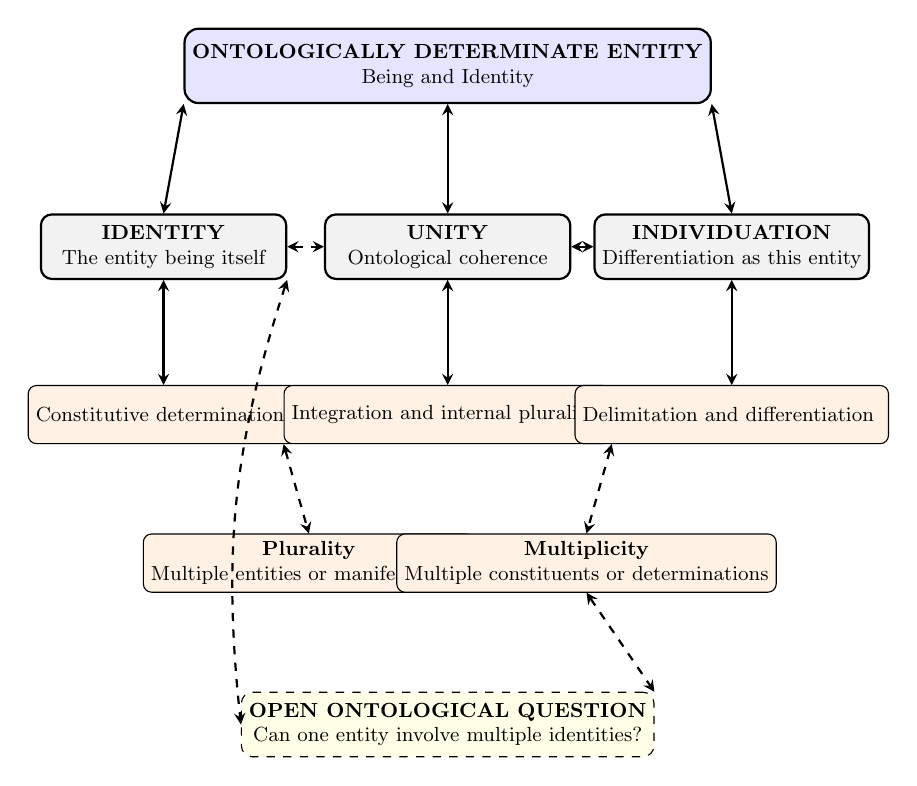
\begin{tikzpicture}[
        scale=0.82,
        transform shape,
        every node/.style={font=\small},
        core/.style={
            rectangle,
            rounded corners=5pt,
            draw=black,
            thick,
            minimum width=4.3cm,
            minimum height=1.15cm,
            align=center,
            fill=blue!10
        },
        concept/.style={
            rectangle,
            rounded corners=4pt,
            draw=black,
            thick,
            minimum width=3.8cm,
            minimum height=1cm,
            align=center,
            fill=gray!10
        },
        dimension/.style={
            rectangle,
            rounded corners=3pt,
            draw=black,
            minimum width=3.5cm,
            minimum height=0.9cm,
            align=center,
            fill=orange!10
        },
        openquestion/.style={
            rectangle,
            rounded corners=4pt,
            draw=black,
            dashed,
            minimum width=4.8cm,
            minimum height=1cm,
            align=center,
            fill=yellow!10
        },
        relation/.style={
            <->,
            thick,
            >=stealth
        },
        analytical/.style={
            <->,
            dashed,
            thick,
            >=stealth
        }
    ]

    % Central ontological entity
    \node[core] (entity) at (0,0) {
        \textbf{ONTOLOGICALLY DETERMINATE ENTITY}\\
        Being and Identity
    };

    % Three analytically distinct dimensions
    \node[concept] (identity) at (-4.4,-2.8) {
        \textbf{IDENTITY}\\
        The entity being itself
    };

    \node[concept] (unity) at (0,-2.8) {
        \textbf{UNITY}\\
        Ontological coherence
    };

    \node[concept] (individuation) at (4.4,-2.8) {
        \textbf{INDIVIDUATION}\\
        Differentiation as this entity
    };

    % Dimensions associated with each concept
    \node[dimension] (constitutive) at (-4.4,-5.4) {
        Constitutive determination
    };

    \node[dimension] (coherence) at (0,-5.4) {
        Integration and internal plurality
    };

    \node[dimension] (distinction) at (4.4,-5.4) {
        Delimitation and differentiation
    };

    % Plurality and multiplicity
    \node[dimension] (plurality) at (-2.15,-7.7) {
        \textbf{Plurality}\\
        Multiple entities or manifestations
    };

    \node[dimension] (multiplicity) at (2.15,-7.7) {
        \textbf{Multiplicity}\\
        Multiple constituents or determinations
    };

    % Open ontological question
    \node[openquestion] (question) at (0,-10.2) {
        \textbf{OPEN ONTOLOGICAL QUESTION}\\
        Can one entity involve multiple identities?
    };

    % Relations between the entity and its dimensions
    \draw[relation] (entity.south west) -- (identity.north);
    \draw[relation] (entity.south) -- (unity.north);
    \draw[relation] (entity.south east) -- (individuation.north);

    % Analytical distinctions
    \draw[analytical] (identity.east) -- (unity.west);
    \draw[analytical] (unity.east) -- (individuation.west);

    % Relations to associated dimensions
    \draw[relation] (identity.south) -- (constitutive.north);
    \draw[relation] (unity.south) -- (coherence.north);
    \draw[relation] (individuation.south) -- (distinction.north);

    % Internal plurality and multiplicity
    \draw[analytical] (coherence.south west) -- (plurality.north);
    \draw[analytical] (coherence.south east) -- (multiplicity.north);

    % The open question is not presented as a settled conclusion
    \draw[analytical] (identity.south east) to[bend right=12]
        (question.west);

    \draw[analytical] (multiplicity.south) -- (question.north east);

    \end{tikzpicture}

    \caption{The Relations Among Identity, Unity, and Individuation: Their Distinct Ontological Dimensions and the Open Question of Multiple Identities Within One Entity}
    \label{fig:identity-unity-and-individuation}
\end{figure}
